\documentclass[twoside,11pt]{article}
\usepackage[margin=3cm]{geometry}


\usepackage{amsmath}
\usepackage{amssymb}
\usepackage{bm}
\usepackage{natbib}
%\usepackage[style=numeric,natbib=true]{biblatex}


\bibliographystyle{chicago}

\RequirePackage[colorlinks=true,citecolor=blue,allbordercolors={1 1 1}]{hyperref}
%\addbibresource{bibliography.bib}
%\bibliography{bibliography}
\usepackage{todonotes} 

\usepackage{subfig}

\usetikzlibrary{bayesnet,calc,angles,quotes}
\usepackage{tikz-3dplot}
\usetikzlibrary{decorations.pathreplacing}
\usepackage[utf8]{inputenc}

\usepackage{amsthm}
\newtheorem{corollary}{Corollary}
\newtheorem{theorem}{Theorem}
\newtheorem{proposition}{Proposition}
\newtheorem{claim}{Claim}
\newtheorem{definition}{Definition}
\newtheorem{lemma}{Lemma}
\newtheorem{assumption}{Assumption}
\newtheorem{problem}{Problem}
\newtheorem{example}{Example}


%\DeclareMathOperator{\dim}{\mathrm{dim}}
\DeclareMathOperator{\Tr}{Tr}
\DeclareMathOperator{\St}{St}
\DeclareMathOperator{\Sp}{\mathrm{Sp}}
\DeclareMathOperator{\Diam}{\mathrm{Diam}}
\DeclareMathOperator{\Diag}{\mathrm{Diag}}
\DeclareMathOperator{\rank}{\mathrm{rk}}
\DeclareMathOperator{\Det}{Det}
\DeclareMathOperator{\Vol}{Vol}
\DeclareMathOperator{\Adj}{Adj}
\DeclareMathOperator{\Span}{\mathrm{Span}}
\DeclareMathOperator{\Conf}{\mathrm{Conf}}
\DeclareMathOperator{\Fr}{\mathrm{Fr}}
\DeclareMathOperator{\DPP}{\mathrm{DPP}}
\DeclareMathOperator{\Cor}{\mathrm{Cor}}
\DeclareMathOperator{\VS}{\mathrm{VS}}
\DeclareMathOperator{\HS}{\mathrm{HS}}
\DeclareMathOperator{\OP}{\mathrm{op}}
\DeclareMathOperator{\eff}{\mathrm{eff}}
\DeclareMathOperator{\Tran}{\intercal}
\newcommand{\dataset}{{\cal D}}
\newcommand{\fracpartial}[2]{\frac{\partial #1}{\partial  #2}}
\DeclareMathOperator{\EX}{\mathbb{E}}
\DeclareMathOperator{\Var}{\mathbb{V}}
\DeclareMathOperator{\Prb}{\mathbb{P}}
\DeclareMathOperator*{\argmax}{arg\,max}
\DeclareMathOperator*{\argmin}{arg\,min}
\DeclareMathOperator*{\KDPP}{\mathfrak{K}}

\DeclareMathOperator{\F}{\mathcal{F}}
\DeclareMathOperator{\X}{\mathcal{X}}
% Expectation symbol


\newcommand{\ab}[1]{\textcolor{red}{#1}}
\newcommand{\pc}[1]{\textcolor{blue}{#1}}
\newcommand{\rb}[1]{\textcolor{magenta}{#1}}


\usepackage{bbold}
% Definitions of handy macros can go here



% Expectation symbol

%\DeclareRobustCommand{\bbone}{\text{\usefont{U}{bbold}{m}{n}1}}


% Heading arguments are {volume}{year}{pages}{date submitted}{date published}{paper id}{author-full-names}



% Short headings should be running head and authors last names

%\firstpageno{1}

\begin{document}

\title{Thesis manuscript}


\author{Ayoub Belhadji} %if necessary, replace with your course title
 
\maketitle
%\author{\name Authors}

%\editor{Editors}

%\maketitle

%\begin{abstract}%   <- trailing '%' for backward compatibility of .sty file
%aaa
%\end{abstract}



\newpage
%\section{Introduction en français}
\section{Introduction}
\subsection{Sensing on budget} 
(3 pages)
\subsection{Design problems in applied mathematics}
(3-6 pages)
\subsection{Mathematical framework: Determinantal point processes}
(7-10 pages)
  Determinantal Point Processes (DPPs) were introduced by \cite{Mac75} as probabilistic models for beams of fermions in quantum optics. Since then, DPPs have been thoroughly studied in random matrix theory \citep{Joh05}, and have more recently been adopted in machine learning \citep*{KuTa12}, spatial statistics \citep*{LaMoRu15}, and Monte Carlo methods \citep{BaHa16}.

The negative correlation property manifested by a large class of DPPs seems appealing to use in design problems. Indeed, one may expect to reduce the sensing budget if the design avoids redundancy and allows to capture the essential of the information. 
Another appealing aspect about DPPs is the possibility of numerically simulate these probabilistic models as several numerical simulation algorithms were proposed and analyzed recently. This make these models amenable to empirical investigations.
 

This thesis is devoted to investigate the suitability of using Determinantal Point Processes (DPPs) as models for randomized designs adapted to the applications evoked previously.

A brief introduction to the theory of DPPs is given in the following. As a probabilistic model, DPPs appear in two forms: discrete DPPs and continuous DPPs. This does not prevent us from giving a unified definition of the two forms. We shall see in the end of this section that these two forms deal with two different approximation problems. Moreover, the two forms diverges regarding the efficiency of the numerical simulations.

Before giving the definitions of DPPs, we recall some basic properties of determinant that are connected to the geometric notion of volume.

\subsubsection{The determinant and the volume}
We recall this elementary result:
\begin{theorem}
Let $...$ be a parallelepiped ... and denote by $\bm{X}$ the matrix ....
Then
\begin{equation}
\Det \bm{X} \bm{X}^{\Tran} = Vol^{2} \mathcal{P}
\end{equation}
\end{theorem}

% Wh a unified definition can be given for these two forms,  can be defined using the same mathematical framework; the accomplished tasks are fundamentally different.





\subsubsection{Definitions}
Before giving the definition of a determinantal point process, we recall briefly the definition of a point process, and we refer to Appendix ?? for further details on this topic.

Intuitively, a point process is a random subset on some set $\X$. Examples of $\X$ include discrete sets (finite or infinite), $\mathbb{R}^{d}$ or some subset of $\mathbb{R}^{d}$ or the hypersphere $\mathbb{S}^{d-1}$. Keeping these examples in mind, we can assume that $\X$ is a separable Hausdorff space.


First, we give the definition of a point process. 

\begin{definition}
A configuration of $\X$ is a subset $\gamma$ of $\X$ that satisfies the following conditions:
\begin{itemize}
\item $\gamma$ is discrete 
\item for every compact subset $\mathcal{K}$ of $\X, \: |\gamma \cap \mathcal{K}| < +\infty $.

\end{itemize}
We denote by $\Gamma$ the set of configurations on $\X$.
\end{definition}

Denote by $\mathcal{G}$, the $\sigma$-algebra generated by the sets 
\begin{equation}
\{\gamma \in \Gamma, \: |\gamma \cap \mathcal{K}| = m \},
\end{equation}
where $\mathcal{K}$ is a compact set of $\X$ and $m \in \mathbb{N}$.



\begin{definition}
A point process $\gamma$ is a measurable application from a measure space into $(\Gamma, \mathcal{G})$.
\end{definition}

In other words, a point process is a random configuration.  

\begin{definition}
Let $\gamma$ be a point process on $\X$, and $n \in \mathbb{N}^{*}$. If there exists a non-negative function $\rho_{n}: \X^{n} \rightarrow \mathbb{R} $ satisfying 
\begin{equation}\label{eq:def_joint_intensity}
\EX \sum\limits_{(x_{1}, \dots, x_{n}) \in \gamma } f(x_{1}, \dots, x_{n}) = \frac{1}{N!} \int_{\X^{N}} f(x_{1}, \dots, x_{n}) \rho_{n}(x_{1}, \dots, x_{n}) \otimes_{i \in [n]} \mathrm{d}\omega(x_{i}),
\end{equation}
for all .... functions $f$, then $\rho_{n}$ is called the $n$-order joint intensity function of $\gamma$.
\end{definition}
By considering a test function $f = \mathbb{1}_{\mathcal{B}}$, \eqref{eq:def_joint_intensity} is equivalent to 
\begin{equation}
\Prb \bigg(\big(x_{1}, \dots, x_{n} \big) \in \mathcal{B} \bigg) = \int_{\mathcal{B}} \rho_{n}(x_{1}, \dots, x_{n}) \otimes_{i \in [n]}\mathrm{d}\omega(x_{i}).
\end{equation}
In other words, $\rho_{n}(x_{1}, \dots, x_{n}) \otimes_{i \in [n]}\mathrm{d}\omega(x_{i})$ is the probability of the event $\big(x_{1}, \dots, x_{n} \big)...$...
In the case $n = 1$, $\rho$

We refer to [??] for further properties on point processes.


A DPP is a point process such that have $n$-order joint intensities, and those intensities are expressed with respect to some kernel $k$.
\begin{definition}\label{eq:def_dpp}
Let $\gamma$ be a point process. $\gamma$ is said to be a determinantal point process on $\X$ with respect to the kernel $k$ and the reference measure $\mathrm{d}\omega$ if its joint densities exist and satisfy
\begin{equation}
\rho_{n}(x_{1}, \dots, x_{n}) = \Det \bm{K}(\bm{x}).
\end{equation}
\end{definition}

In the definition~\eqref{eq:def_dpp}, the kernel $k$ governs the statistical properties of the point process $\gamma$. For instance, if $n =1$, ...

In this section, we introduce discrete determinantal point processes (DPPs) and the related $k$-DPPs, of which volume sampling is an example. 


For all the definitions in this section, we refer the reader to \citep{KuTa12}. Recall that $[d] = \{1,\dots,d\}$.% A point process on $[d]$ is a probability measure over subsets of $[d]$.
\begin{definition}[DPP]
Let $\bm{K} \in \mathbb{R}^{d\times d}$ be a positive semi-definite matrix.
A random subset $Y \subseteq [d]$ is drawn from a DPP of marginal kernel $\bm{K}$ if and only if
\begin{equation}\label{eq:def_dpp}
\forall S \subseteq [d],\quad \Prb(S \subseteq Y) = \Det(\bm{K}_{S}),
\end{equation}
where $\bm{K}_{S} = [\bm{K}_{i,j}]_{i,j \in S}$. We take as a convention $\Det(\bm{K}_{\emptyset}) = 1$.
\end{definition}
%In this paper, we use a definition of DPPs through their ...
%Note that it is also common to see in the literature a related definition called an $\bm{L}$-ensemble \citet{KuTa12}.
For a given matrix $\bm{K}$, it is not obvious that \eqref{eq:def_dpp} consistently defines a point process. One sufficient condition is that $\bm{K}$ is symmetric and its spectrum is in $[0,1]$; see \citep{Mac75} and \citep{Sos00}[Theorem 3]. In particular, when the spectrum of $\bm{K}$ is included in $\{0,1\}$, we call $\bm{K}$ a projection kernel and the corresponding DPP a \emph{projection} DPP\footnote{All projection DPPs in this paper have symmetric kernels}. Letting $r$ be the number of unit eigenvalues of its kernel, samples from a projection DPP have fixed cardinality $r$ with probability 1 \cite*[Lemma 17]{HoKrPeVi06}.

For symmetric kernels $\bm{K}$, a DPP can be seen as a \emph{repulsive} distribution, in the sense that for all $i,j\in [d]$,
\begin{align}
  \Prb(\{i,j\} \subseteq Y) &= \bm{K}_{i,i} \bm{K}_{j,j} - \bm{K}^2_{i,j}\\
  &= \Prb(\{i\} \subseteq Y)\Prb(\{j\} \subseteq Y) - \bm{K}^2_{i,j}\\
  &\leq \Prb(\{i\} \subseteq Y)\Prb(\{j\} \subseteq Y).
\end{align}

Besides projection DPPs, there is another natural way of using a kernel matrix to define a random subset of $[d]$ with prespecified cardinality $k$.
\begin{definition}[$k$-DPP]\label{def:kDPP}
Let $\bm{L} \in \mathbb{R}^{d\times d}$ be a positive semidefinite matrix.
A random subset $Y \subseteq [d]$ is drawn from a $k$-DPP of kernel $\bm{L}$ if and only if
\begin{equation}\label{eq:def_kdpp}
\forall S \subseteq [d],\quad \Prb(Y = S) \propto \mathbb{1}_{\{\vert S\vert = k\}}\Det(\bm{L}_{S})
\end{equation}
where $\bm{L}_{S} = [\bm{L}_{i,j}]_{i,j \in S}$.
\end{definition}
DPPs and $k$-DPPs are closely related but different objects. For starters, $k$-DPPs are always well-defined provided $\bm{L}$ has a nonzero minor of size $k$.

\subsection{Sampling from a DPP and a $k$-DPP}
\label{subsec:sampling_from_a_dpp}
Let $\bm{K}\in\mathbb{R}^{d\times d}$ be a symmetric, positive semi-definite matrix, with eigenvalues in $[0,1]$, so that $\bm{K}$ is the marginal kernel of a DPP on $[d]$. Let us diagonalize it as $\bm{K} = \bm{V}\text{Diag}(\lambda_i)\bm{V}^{\Tran}$. \cite{HoKrPeVi06} established that sampling from the DPP with kernel $\bm K$ can be done by \emph{(i)} sampling independent Bernoulli $B_i, i=1,\dots,d$, with respective parameters $\lambda_i$, \emph{(ii)} forming the submatrix $\bm V_{:,B}$ of $\bm V$ corresponding to columns $i$ such that $B_i=1$, and \emph{(iii)} sampling from the projection DPP with kernel
$$\bm{K}_\text{proj} = \bm{V}_{:,B}\bm{V}_{:,B}^{\Tran}.$$
The only nontrivial step is sampling from a projection DPP, for which we give pseudocode in Figure~\ref{alg:DPP_SAMPLER}; see \cite[Theorem 7]{HoKrPeVi06} or \cite[Theorem 2.3]{KuTa12} for a proof. For a survey of variants of the algorithm, we also refer to \citep*{TrBaAm18} and the documentation of the DPPy toolbox\footnote{\url{http://github.com/guilgautier/DPPy}} \citep*{GaBaVa18}. For our purposes, it is enough to remark that general DPPs are mixtures of projection DPPs of different ranks, and that the cardinality of a general DPP is a sum of independent Bernoulli random variables.

% \begin{figure}[!ht]
% \centerline{
% \scalebox{0.9}{
% \begin{algorithm}{$\Algo{ProjectionDPP}\big(\bm{K}_\text{proj}=\bm{V}\bm{V}^{\Tran})$}
% %\vspace{-.1cm}
% \Aitem $Y \longleftarrow  \emptyset$
% \Aitem $\bm{W} \longleftarrow  \bm{V}$
% \Aitem \While $\text{rk}(\bm{W}) > 0 $
% \Aitem \mt  Sample $i$ from $\Omega$ with probability $ \propto \|\bm{W}_{i,:}\|_{2}^{2}$ \ar{Chain rule}
% \Aitem \mt  $Y \longleftarrow  Y \cup \{i\}$
% \Aitem \mt $\bm{V} \longleftarrow \bm{V}_{\perp}$ an orthonormal basis of $\Span(\bm{V} \cap \bm{e}_{i}^{\perp})$
% \Aitem \Return $Y$
% \end{algorithm}
% }
% }
% \caption{Pseudocode for sampling from a DPP of marginal kernel $\bm{K}$.}
% \label{alg:DPP_SAMPLER}
% \end{figure}

The next proposition establishes that $k$-DPPs also are mixtures of projection DPPs.
\begin{proposition}(\citet[Section 5.2.2]{KuTa12})
\label{prop:kdpp_mixture_proposition}
Let $Y$ be a random subset of $[d]$ sampled from a $k$-DPP with kernel $\bm{L}$. We further assume that $\bm L$ is symmetric, we denote its rank by $r$ and its diagonalization by $\bm L = \bm{V}\bm{\Lambda}\bm{V}^{\Tran}$. Finally, let $k\leq r$. It holds
\begin{equation}
\label{eq:volume_sampling_as_mixture_equation}
\Prb(Y = S) = \sum\limits_{\substack{T \subseteq [r]\\|T| = k}} \mu_{T} \left[\frac{1}{k!} \Det\left(\bm{V}_{T,S}\bm{V}^{\Tran}_{T,S}\right)\right]
\end{equation}
where
\begin{equation}
\mu_{T} = \frac{\prod_{i \in T}\lambda_{i}}{\sum\limits_{\substack{U \subseteq[r]\\ |U| = k}}\prod_{i \in U}\lambda_{i}}.
\label{e:kDPPWeights}
\end{equation}
\end{proposition}
Each mixture component in square brackets in \eqref{eq:volume_sampling_as_mixture_equation} is a projection DPP with cardinality $k$. Sampling a $k$-DPP can thus be done by \emph{(i)} sampling a multinomial distribution with parameters \eqref{e:kDPPWeights}, and \emph{(ii)} sampling from the corresponding projection DPP using the algorithm in Figure~\ref{alg:DPP_SAMPLER}. The main difference between $k$-DPPs and DPPs is that all mixture components in \eqref{eq:volume_sampling_as_mixture_equation} have the same cardinality $k$. In particular, projection DPPs are the only DPPs that are also $k$-DPPs.
%\begin{algorithm}[H]
%\SetAlgoLined
%\KwData{The kernel $L$}
%$(\Lambda,\bm{V}) \longleftarrow eigen(\bm{L})$\\
%$T \longleftarrow  \emptyset$\\
%$Y \longleftarrow  \emptyset$\\

%Sample T, $k$ eigenvectors of $\bm{K}$, with probability $\Prb(T) \propto \prod_{i \in T}\lambda_{i}$\\
%Sample Y, with probability $\Prb(Y) = \Det(\bm{V}_{T,Y}\bm{V}_{T,Y}^{\Tran})$ using Algorithm \ref{alg:dpp_sampler_algorithm}\\
%\KwResult{Y}
%\caption{Sampling from a $k$-DPP}
%\end{algorithm}
% \begin{figure}[!ht]
% \centerline{
% \scalebox{0.9}{
% \begin{algorithm}{$\Algo{k-DPP}\big(\bm{L})$}
% %\vspace{-.1cm}
% \Aitem $(\bm{V},\bm{\Lambda}) \longleftarrow \text{eig}(\bm{L})$
% \Aitem $Y \longleftarrow  \emptyset$
% \Aitem Sample $T \subseteq [r], |T| = k$ such that $\Prb(T) \propto \frac{\prod_{i \in T}\lambda_{i}}{\sum\limits_{U \subseteq[r],|U| = k}\prod_{i \in U}\lambda_{i}}$
% \Aitem $s\bm{V} \longleftarrow  \bm{V}_{:,T}$
% %$$
% \Aitem \While $\text{rk}(s\bm{V}) > 0 $
% \Aitem \mt  Sample $i$ from $\Omega$ with probability $\Prb(i) \propto \|s\bm{V}_{i,:}\|_{2}^{2}$
% \Aitem \mt  $Y \longleftarrow  Y \cup \{i\}$
% \Aitem \mt $\bm{V} \longleftarrow \bm{V}_{\perp}$ an orthonormal basis of $Span(\bm{V} \cap \bm{e}_{i}^{\perp})$
% \Aitem \Return $Y$
% \end{algorithm}
% }
% }
% \caption{Pseudocode of sampling from a k-DPP of kernel $\bm{L}$.}
% \label{f:DPP_SAMPLER}
% \end{figure}
% \begin{figure}[!ht]
%   \centering
% %  \subfigure[SVD]{
%      \subfloat[SVD of $\bm{X}$]{\input{img/colorful_svd.tex}}\\
%      \subfloat[Sampling $k$ columns according to VS and our DPP]{

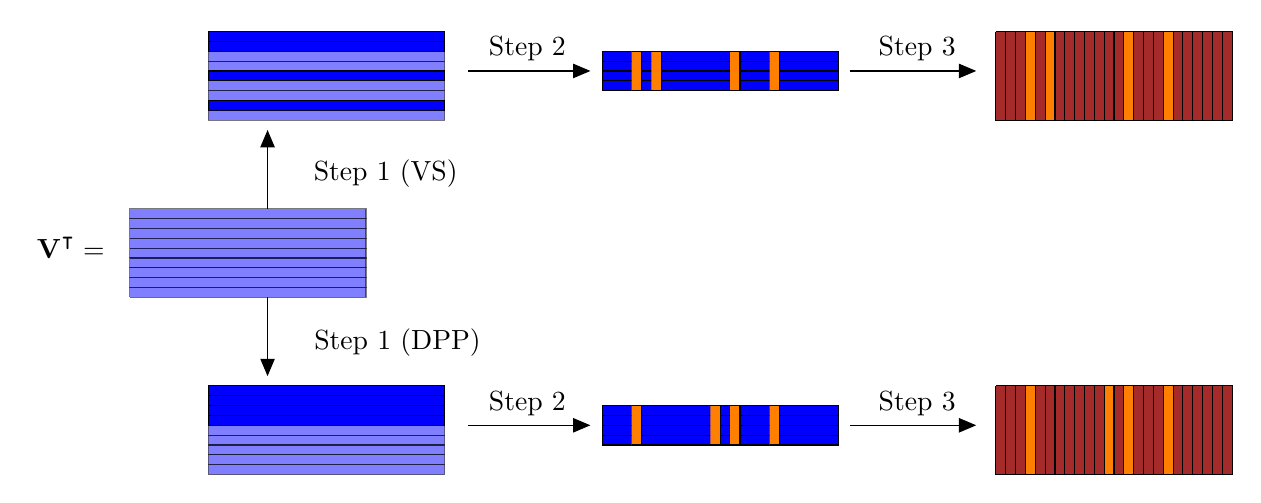
\begin{tikzpicture}[scale = 0.5]

  % draw line and angle
%  \draw
%     pic [draw,angle radius=4mm,angle eccentricity=1.5, "$\theta$" font=\scriptsize] {angle=v2--v1--v3};
\begin{scope}[yshift=-45mm]
\begin{scope}[xshift=-20mm]

\draw [fill=blue, opacity=0.5] (-16,3.75) -- (-10,3.75) -- (-10,4) -- (-16,4) -- (-16,3.75);
\draw [fill=blue, opacity=0.5] (-16,3.5) -- (-10,3.5) -- (-10,3.75) -- (-16,3.75) -- (-16,3.5);
\draw [fill=blue, opacity=0.5] (-16,3.25) -- (-10,3.25) -- (-10,3.5) -- (-16,3.5) -- (-16,3.25);
\draw [fill=blue, opacity=0.5] (-16,3) -- (-10,3) -- (-10,3.25) -- (-16,3.25) -- (-16,3);
\draw [fill=blue, opacity=0.5] (-16,2.75) -- (-10,2.75) -- (-10,3) -- (-16,3) -- (-16,2.75);
\draw [fill=blue, opacity=0.5] (-16,2.5) -- (-10,2.5) -- (-10,2.75) -- (-16,2.75) -- (-16,2.5);
\draw [fill=blue, opacity=0.5] (-16,2.25) -- (-10,2.25) -- (-10,2.5) -- (-16,2.5) -- (-16,2.25);
\draw [fill=blue, opacity=0.5] (-16,2) -- (-10,2) -- (-10,2.25) -- (-16,2.25) -- (-16,2);
\draw [fill=blue, opacity=0.5] (-16,1.75) -- (-10,1.75) -- (-10,2) -- (-16,2) -- (-16,1.75);


\draw  (-17.5,2.5)  node [above ] {$\bm{\mathrm{V}}^{\Tran} = $} ;

\draw  (-9.5,4.3)  node [above ] {Step 1 (VS)} ;

\draw [->] (-12.5,4) --  (-12.5,6);


\draw  (-9.2,0)  node [above ] {Step 1 (DPP)} ;

\draw [->] (-12.5,1.75) --  (-12.5,-0.25);

\end{scope}
\end{scope}





\begin{scope}[xshift=-120mm]


\draw [fill=blue, opacity=1] (-4,3.75) -- (2,3.75) -- (2,4) -- (-4,4) -- (-4,3.75);
\draw [fill=blue, opacity=1] (-4,3.5) -- (2,3.5) -- (2,3.75) -- (-4,3.75) -- (-4,3.5);
\draw [fill=blue, opacity=0.5] (-4,3.25) -- (2,3.25) -- (2,3.5) -- (-4,3.5) -- (-4,3.25);
\draw [fill=blue, opacity=0.5] (-4,3) -- (2,3) -- (2,3.25) -- (-4,3.25) -- (-4,3);
\draw [fill=blue, opacity=1] (-4,2.75) -- (2,2.75) -- (2,3) -- (-4,3) -- (-4,2.75);
\draw [fill=blue, opacity=0.5] (-4,2.5) -- (2,2.5) -- (2,2.75) -- (-4,2.75) -- (-4,2.5);
\draw [fill=blue, opacity=0.5] (-4,2.25) -- (2,2.25) -- (2,2.5) -- (-4,2.5) -- (-4,2.25);
\draw [fill=blue, opacity=1] (-4,2) -- (2,2) -- (2,2.25) -- (-4,2.25) -- (-4,2);
\draw [fill=blue, opacity=0.5] (-4,1.75) -- (2,1.75) -- (2,2) -- (-4,2) -- (-4,1.75);



\draw [->] (2.6,3) --  (4.1,3)  node [above] { Step 2 } --  (5.7,3);


\end{scope}


\begin{scope}[xshift=-120mm]
\begin{scope}[yshift=-90mm]


\draw [fill=blue, opacity=1] (-4,3.75) -- (2,3.75) -- (2,4) -- (-4,4) -- (-4,3.75);
\draw [fill=blue, opacity=1] (-4,3.5) -- (2,3.5) -- (2,3.75) -- (-4,3.75) -- (-4,3.5);
\draw [fill=blue, opacity=1] (-4,3.25) -- (2,3.25) -- (2,3.5) -- (-4,3.5) -- (-4,3.25);
\draw [fill=blue, opacity=1] (-4,3) -- (2,3) -- (2,3.25) -- (-4,3.25) -- (-4,3);
\draw [fill=blue, opacity=0.5] (-4,2.75) -- (2,2.75) -- (2,3) -- (-4,3) -- (-4,2.75);
\draw [fill=blue, opacity=0.5] (-4,2.5) -- (2,2.5) -- (2,2.75) -- (-4,2.75) -- (-4,2.5);
\draw [fill=blue, opacity=0.5] (-4,2.25) -- (2,2.25) -- (2,2.5) -- (-4,2.5) -- (-4,2.25);
\draw [fill=blue, opacity=0.5] (-4,2) -- (2,2) -- (2,2.25) -- (-4,2.25) -- (-4,2);
\draw [fill=blue, opacity=0.5] (-4,1.75) -- (2,1.75) -- (2,2) -- (-4,2) -- (-4,1.75);



\draw [->] (2.6,3) --  (4.1,3)  node [above] { Step 2 } --  (5.7,3);


\end{scope}
\end{scope}


\begin{scope}[xshift=-145mm]

\draw [fill=blue, opacity=1] (8.5,3.25) -- (14.5,3.25) -- (14.5,3.5) -- (8.5,3.5) -- (8.5,3.25);
\draw [fill=blue, opacity=1] (8.5,3) -- (14.5,3) -- (14.5,3.25) -- (8.5,3.25) -- (8.5,3);
\draw [fill=blue, opacity=1] (8.5,2.75) -- (14.5,2.75) -- (14.5,3) -- (8.5,3) -- (8.5,2.75);
\draw [fill=blue, opacity=1] (8.5,2.5) -- (14.5,2.5) -- (14.5,2.75) -- (8.5,2.75) -- (8.5,2.5);


\draw [fill=orange, opacity=1] (9.25,2.5) -- (9.25,2.5) -- (9.5,2.5) -- (9.5,3.5) -- (9.25,3.5);
\draw [fill=orange, opacity=1] (9.75,2.5) -- (9.75,2.5) -- (10,2.5) -- (10,3.5) -- (9.75,3.5);
\draw [fill=orange, opacity=1] (11.75,2.5) -- (11.75,2.5) -- (12,2.5) -- (12,3.5) -- (11.75,3.5);
\draw [fill=orange, opacity=1] (12.75,2.5) -- (12.75,2.5) -- (13,2.5) -- (13,3.5) -- (12.75,3.5);



\draw [->] (14.8,3) --  (16.5,3)  node [above] { Step 3 } --  (18,3);

\end{scope}

\begin{scope}[yshift=-90mm]
\begin{scope}[xshift=-145mm]

\draw [fill=blue, opacity=1] (8.5,3.25) -- (14.5,3.25) -- (14.5,3.5) -- (8.5,3.5) -- (8.5,3.25);
\draw [fill=blue, opacity=1] (8.5,3) -- (14.5,3) -- (14.5,3.25) -- (8.5,3.25) -- (8.5,3);
\draw [fill=blue, opacity=1] (8.5,2.75) -- (14.5,2.75) -- (14.5,3) -- (8.5,3) -- (8.5,2.75);
\draw [fill=blue, opacity=1] (8.5,2.5) -- (14.5,2.5) -- (14.5,2.75) -- (8.5,2.75) -- (8.5,2.5);


\draw [fill=orange, opacity=1] (9.25,2.5) -- (9.25,2.5) -- (9.5,2.5) -- (9.5,3.5) -- (9.25,3.5);
\draw [fill=orange, opacity=1] (11.25,2.5) -- (11.25,2.5) -- (11.5,2.5) -- (11.5,3.5) -- (11.25,3.5);
\draw [fill=orange, opacity=1] (11.75,2.5) -- (11.75,2.5) -- (12,2.5) -- (12,3.5) -- (11.75,3.5);
\draw [fill=orange, opacity=1] (12.75,2.5) -- (12.75,2.5) -- (13,2.5) -- (13,3.5) -- (12.75,3.5);



\draw [->] (14.8,3) --  (16.5,3)  node [above] { Step 3 } --  (18,3);

\end{scope}
\end{scope}

%\begin{scope}[yshift=-45mm]
\begin{scope}[xshift=200mm]
 

\draw [fill=Brown, opacity=1] (-16,4) -- (-15.75,4) -- (-15.75,1.75) -- (-16,1.75) -- (-16,4);
\draw [fill=Brown, opacity=1] (-15.75,4) -- (-15.5,4) -- (-15.5,1.75) -- (-15.75,1.75) -- (-15.75,4);

\draw [fill=Brown, opacity=1] (-15.5,4) -- (-15.25,4) -- (-15.25,1.75) -- (-15.5,1.75) -- (-15.5,4);
\draw [fill=orange, opacity=1] (-15.25,4) -- (-15,4) -- (-15,1.75) -- (-15.25,1.75) -- (-15.25,4);
\draw [fill=Brown, opacity=1] (-15,4) -- (-14.75,4) -- (-14.75,1.75) -- (-15,1.75) -- (-15,4);
\draw [fill=orange, opacity=1] (-14.75,4) -- (-14.5,4) -- (-14.5,1.75) -- (-14.75,1.75) -- (-14.75,4);
\draw [fill=Brown, opacity=1] (-14.5,4) -- (-14.25,4) -- (-14.25,1.75) -- (-14.5,1.75) -- (-14.5,4);
\draw [fill=Brown, opacity=1] (-14.25,4) -- (-14,4) -- (-14,1.75) -- (-14.25,1.75) -- (-14.25,4);
\draw [fill=Brown, opacity=1] (-14,4) -- (-13.75,4) -- (-13.75,1.75) -- (-14,1.75) -- (-14,4);
\draw [fill=Brown, opacity=1] (-13.75,4) -- (-13.5,4) -- (-13.5,1.75) -- (-13.75,1.75) -- (-13.75,4);
\draw [fill=Brown, opacity=1] (-13.5,4) -- (-13.25,4) -- (-13.25,1.75) -- (-13.5,1.75) -- (-13.5,4);
\draw [fill=Brown, opacity=1] (-13.25,4) -- (-13,4) -- (-13,1.75) -- (-13.25,1.75) -- (-13.25,4);
\draw [fill=Brown, opacity=1] (-13,4) -- (-12.75,4) -- (-12.75,1.75) -- (-13,1.75) -- (-13,4);

\draw [fill=orange, opacity=1] (-12.75,4) -- (-12.5,4) -- (-12.5,1.75) -- (-12.75,1.75) -- (-12.75,4);
\draw [fill=Brown, opacity=1] (-12.5,4) -- (-12.25,4) -- (-12.25,1.75) -- (-12.5,1.75) -- (-12.5,4);
\draw [fill=Brown, opacity=1] (-12.25,4) -- (-12,4) -- (-12,1.75) -- (-12.25,1.75) -- (-12.25,4);
\draw [fill=Brown, opacity=1] (-12,4) -- (-11.75,4) -- (-11.75,1.75) -- (-12,1.75) -- (-12,4);

\draw [fill=orange, opacity=1] (-11.75,4) -- (-11.5,4) -- (-11.5,1.75) -- (-11.75,1.75) -- (-11.75,4);
\draw [fill=Brown, opacity=1] (-11.5,4) -- (-11.25,4) -- (-11.25,1.75) -- (-11.5,1.75) -- (-11.5,4);
\draw [fill=Brown, opacity=1] (-11.25,4) -- (-11,4) -- (-11,1.75) -- (-11.25,1.75) -- (-11.25,4);
\draw [fill=Brown, opacity=1] (-11,4) -- (-10.75,4) -- (-10.75,1.75) -- (-11,1.75) -- (-11,4);
\draw [fill=Brown, opacity=1] (-10.75,4) -- (-10.5,4) -- (-10.5,1.75) -- (-10.75,1.75) -- (-10.75,4);
\draw [fill=Brown, opacity=1] (-10.5,4) -- (-10.25,4) -- (-10.25,1.75) -- (-10.5,1.75) -- (-10.5,4);
\draw [fill=Brown, opacity=1] (-10.25,4) -- (-10,4) -- (-10,1.75) -- (-10.25,1.75) -- (-10.25,4);


\end{scope}
%\end{scope}


\begin{scope}[yshift=-90mm]
\begin{scope}[xshift=200mm]
 

\draw [fill=Brown, opacity=1] (-16,4) -- (-15.75,4) -- (-15.75,1.75) -- (-16,1.75) -- (-16,4);
\draw [fill=Brown, opacity=1] (-15.75,4) -- (-15.5,4) -- (-15.5,1.75) -- (-15.75,1.75) -- (-15.75,4);

\draw [fill=Brown, opacity=1] (-15.5,4) -- (-15.25,4) -- (-15.25,1.75) -- (-15.5,1.75) -- (-15.5,4);
\draw [fill=orange, opacity=1] (-15.25,4) -- (-15,4) -- (-15,1.75) -- (-15.25,1.75) -- (-15.25,4);
\draw [fill=Brown, opacity=1] (-15,4) -- (-14.75,4) -- (-14.75,1.75) -- (-15,1.75) -- (-15,4);
\draw [fill=Brown, opacity=1] (-14.75,4) -- (-14.5,4) -- (-14.5,1.75) -- (-14.75,1.75) -- (-14.75,4);
\draw [fill=Brown, opacity=1] (-14.5,4) -- (-14.25,4) -- (-14.25,1.75) -- (-14.5,1.75) -- (-14.5,4);
\draw [fill=Brown, opacity=1] (-14.25,4) -- (-14,4) -- (-14,1.75) -- (-14.25,1.75) -- (-14.25,4);
\draw [fill=Brown, opacity=1] (-14,4) -- (-13.75,4) -- (-13.75,1.75) -- (-14,1.75) -- (-14,4);
\draw [fill=Brown, opacity=1] (-13.75,4) -- (-13.5,4) -- (-13.5,1.75) -- (-13.75,1.75) -- (-13.75,4);
\draw [fill=Brown, opacity=1] (-13.5,4) -- (-13.25,4) -- (-13.25,1.75) -- (-13.5,1.75) -- (-13.5,4);
\draw [fill=orange, opacity=1] (-13.25,4) -- (-13,4) -- (-13,1.75) -- (-13.25,1.75) -- (-13.25,4);
\draw [fill=Brown, opacity=1] (-13,4) -- (-12.75,4) -- (-12.75,1.75) -- (-13,1.75) -- (-13,4);

\draw [fill=orange, opacity=1] (-12.75,4) -- (-12.5,4) -- (-12.5,1.75) -- (-12.75,1.75) -- (-12.75,4);
\draw [fill=Brown, opacity=1] (-12.5,4) -- (-12.25,4) -- (-12.25,1.75) -- (-12.5,1.75) -- (-12.5,4);
\draw [fill=Brown, opacity=1] (-12.25,4) -- (-12,4) -- (-12,1.75) -- (-12.25,1.75) -- (-12.25,4);
\draw [fill=Brown, opacity=1] (-12,4) -- (-11.75,4) -- (-11.75,1.75) -- (-12,1.75) -- (-12,4);

\draw [fill=orange, opacity=1] (-11.75,4) -- (-11.5,4) -- (-11.5,1.75) -- (-11.75,1.75) -- (-11.75,4);
\draw [fill=Brown, opacity=1] (-11.5,4) -- (-11.25,4) -- (-11.25,1.75) -- (-11.5,1.75) -- (-11.5,4);
\draw [fill=Brown, opacity=1] (-11.25,4) -- (-11,4) -- (-11,1.75) -- (-11.25,1.75) -- (-11.25,4);
\draw [fill=Brown, opacity=1] (-11,4) -- (-10.75,4) -- (-10.75,1.75) -- (-11,1.75) -- (-11,4);
\draw [fill=Brown, opacity=1] (-10.75,4) -- (-10.5,4) -- (-10.5,1.75) -- (-10.75,1.75) -- (-10.75,4);
\draw [fill=Brown, opacity=1] (-10.5,4) -- (-10.25,4) -- (-10.25,1.75) -- (-10.5,1.75) -- (-10.5,4);
\draw [fill=Brown, opacity=1] (-10.25,4) -- (-10,4) -- (-10,1.75) -- (-10.25,1.75) -- (-10.25,4);


\end{scope}
\end{scope}

% \begin{scope}[xshift=-50mm]





% \end{scope}

%\draw  (23,2)  node [above] {Complexity } ;

\end{tikzpicture}
}
%   %  \subfloat[]{

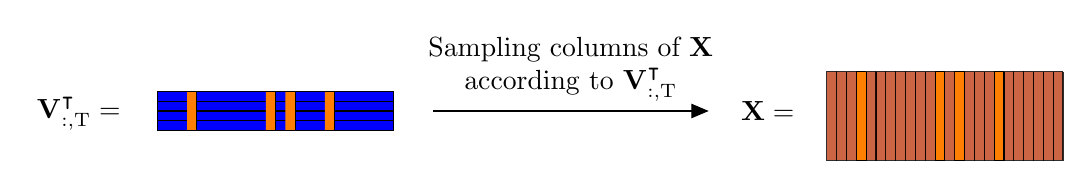
\begin{tikzpicture}[scale = 0.5]

  % draw line and angle
%  \draw 
%     pic [draw,angle radius=4mm,angle eccentricity=1.5, "$\theta$" font=\scriptsize] {angle=v2--v1--v3};

\begin{scope}[xshift=-65mm]



\draw [fill=blue, opacity=1] (0.5,3.25) -- (6.5,3.25) -- (6.5,3.5) -- (0.5,3.5) -- (0.5,3.25);
\draw [fill=blue, opacity=1] (0.5,3) -- (6.5,3) -- (6.5,3.25) -- (0.5,3.25) -- (0.5,3);
\draw [fill=blue, opacity=1] (0.5,2.75) -- (6.5,2.75) -- (6.5,3) -- (0.5,3) -- (0.5,2.75);
\draw [fill=blue, opacity=1] (0.5,2.5) -- (6.5,2.5) -- (6.5,2.75) -- (0.5,2.75) -- (0.5,2.5);


\draw [fill=orange, opacity=1] (1.25,2.5) -- (1.25,2.5) -- (1.5,2.5) -- (1.5,3.5) -- (1.25,3.5);
\draw [fill=orange, opacity=1] (3.25,2.5) -- (3.25,2.5) -- (3.5,2.5) -- (3.5,3.5) -- (3.25,3.5);
\draw [fill=orange, opacity=1] (3.75,2.5) -- (3.75,2.5) -- (4,2.5) -- (4,3.5) -- (3.75,3.5);
\draw [fill=orange, opacity=1] (4.75,2.5) -- (4.75,2.5) -- (5,2.5) -- (5,3.5) -- (4.75,3.5);


 \draw  (-1.5,2.25)  node [above] {$\bm{\mathrm{V}}_{:,\mathrm{T}}^{\Tran}=$} ;
\end{scope}

\begin{scope}[xshift=10mm]


\draw [fill=Bittersweet, opacity=0.8] (16,4) -- (15.75,4) -- (15.75,1.75) -- (16,1.75) -- (16,4);
\draw [fill=Bittersweet, opacity=0.8] (15.75,4) -- (15.5,4) -- (15.5,1.75) -- (15.75,1.75) -- (15.75,4);

\draw [fill=Bittersweet, opacity=0.8] (15.5,4) -- (15.25,4) -- (15.25,1.75) -- (15.5,1.75) -- (15.5,4);
\draw [fill=Bittersweet, opacity=0.8] (15.25,4) -- (15,4) -- (15,1.75) -- (15.25,1.75) -- (15.25,4);
\draw [fill=Bittersweet, opacity=0.8] (15,4) -- (14.75,4) -- (14.75,1.75) -- (15,1.75) -- (15,4);
\draw [fill=Bittersweet, opacity=0.8] (14.75,4) -- (14.5,4) -- (14.5,1.75) -- (14.75,1.75) -- (14.75,4);
\draw [fill=orange, opacity=1] (14.5,4) -- (14.25,4) -- (14.25,1.75) -- (14.5,1.75) -- (14.5,4);
\draw [fill=Bittersweet, opacity=0.8] (14.25,4) -- (14,4) -- (14,1.75) -- (14.25,1.75) -- (14.25,4);
\draw [fill=Bittersweet, opacity=0.8] (14,4) -- (13.75,4) -- (13.75,1.75) -- (14,1.75) -- (14,4);
\draw [fill=Bittersweet, opacity=0.8] (13.75,4) -- (13.5,4) -- (13.5,1.75) -- (13.75,1.75) -- (13.75,4);
\draw [fill=orange, opacity=1] (13.5,4) -- (13.25,4) -- (13.25,1.75) -- (13.5,1.75) -- (13.5,4);
\draw [fill=Bittersweet, opacity=0.8] (13.25,4) -- (13,4) -- (13,1.75) -- (13.25,1.75) -- (13.25,4);
\draw [fill=orange, opacity=1] (13,4) -- (12.75,4) -- (12.75,1.75) -- (13,1.75) -- (13,4);

\draw [fill=Bittersweet, opacity=0.8] (12.75,4) -- (12.5,4) -- (12.5,1.75) -- (12.75,1.75) -- (12.75,4);
\draw [fill=Bittersweet, opacity=0.8] (12.5,4) -- (12.25,4) -- (12.25,1.75) -- (12.5,1.75) -- (12.5,4);
\draw [fill=Bittersweet, opacity=0.8] (12.25,4) -- (12,4) -- (12,1.75) -- (12.25,1.75) -- (12.25,4);
\draw [fill=Bittersweet, opacity=0.8] (12,4) -- (11.75,4) -- (11.75,1.75) -- (12,1.75) -- (12,4);

\draw [fill=Bittersweet, opacity=0.8] (11.75,4) -- (11.5,4) -- (11.5,1.75) -- (11.75,1.75) -- (11.75,4);
\draw [fill=Bittersweet, opacity=0.8] (11.5,4) -- (11.25,4) -- (11.25,1.75) -- (11.5,1.75) -- (11.5,4);
\draw [fill=Bittersweet, opacity=0.8] (11.25,4) -- (11,4) -- (11,1.75) -- (11.25,1.75) -- (11.25,4);
\draw [fill=orange, opacity=1] (11,4) -- (10.75,4) -- (10.75,1.75) -- (11,1.75) -- (11,4);
\draw [fill=Bittersweet, opacity=0.8] (10.75,4) -- (10.5,4) -- (10.5,1.75) -- (10.75,1.75) -- (10.75,4);
\draw [fill=Bittersweet, opacity=0.8] (10.5,4) -- (10.25,4) -- (10.25,1.75) -- (10.5,1.75) -- (10.5,4);
\draw [fill=Bittersweet, opacity=0.8] (10.25,4) -- (10,4) -- (10,1.75) -- (10.25,1.75) -- (10.25,4);


\draw  (8.5,2.5)  node [above] {$\bm{\mathrm{X}} = $} ;
\end{scope}


\draw [->] (1,3) --  (4.5,3)  node [above] {} --  (8,3);

\draw  (4.5,3)  node [above , align=center] {Sampling columns of $\bm{\mathrm{X}}$\\ according to $\bm{\mathrm{V}}_{:,\mathrm{T}}^{\Tran}$} ;



% \draw [->] (-9.5,3) --  (-7.5,3)  node [above] { $\Prb(T)$} --  (-5,3);

% \draw [->] (3,3) --  (5,3)  node [above] { $\Prb(S|T)$} --  (7.5,3);


% \draw  (-7.5,4.25)  node [above] {Step 1} ;

% \draw  (5,4.25)  node [above] {Step 2} ;

%\draw  (23,2)  node [above] {Complexity } ;

\end{tikzpicture}
}\\
%     %\caption{DPP sampling algorithm
%     %\label{f:dpp_sampling_algorithm}
%     %}
% %    \subfloat[]{\input{img/projection_dpp_sampling_algorithm.tex}}\\
% %\subfloat[]{\input{img/volume_sampling_algorithm.tex}}
%     %\caption{Volume sampling algorithm
%     %label{f:volume_sampling_algorithm}
%     %}
%     \caption{A graphical depiction of the sampling algorithms for volume sampling (VS) and the DPP with marginal kernel $\bm{V}^{}_{k}\bm{V}_{k}^{\Tran}$. (a) Both algorithms start with an SVD. (b) In Step 1, VS randomly selects $k$ rows of $\bm V^{\Tran}$, while our DPP always picks the first $k$ rows. Step 2 is the same for both algorithms: jointly sample $k$ columns of the subsampled $\bm V^{\Tran}$, proportionally to their squared volume. Finally, Step 3 is simply the extraction of the corresponding columns of $\bm X$.
%     %The common steps on the sampling algorithm for DPPs and volume sampling. Step 1: sample a random subset of right eigenvectors $T \subseteq [r]$with probability $\Prb(T)$. Step 2: sample a random subset of columns indices $S \subseteq [d]$ with probability $\Prb(S|T)$.
%     \label{f:sampling}
%     }
% \end{figure}

% \begin{table}
% \centering
%  \begin{tabular}{| c| c| c|}
%  \hline
%   - & Step 1 & Step 2\\
%  \hline
%  Projection DPP & $\Prb(T=[k]) = 1$ & $\Prb(S|T) = \Det (\bm{V}_{S,[k]})^{2}$\\
%  \hline
%  DPP & $\Prb(t \in T) = \lambda_{t}$ & $\Prb(S|T) = \Det (\bm{V}_{S,T})^{2}$\\
%  \hline
%  Volume sampling & $\Prb(T) \propto \prod_{i \in T} \sigma_{i}^{2}$ & $\Prb(S|T) = \Det (\bm{V}_{S,T})^{2}$\\
%  \hline
% \end{tabular}
% \caption{Differences in sampling schemes between projection DPP, DPP and volume sampling.}
% \end{table}

A fundamental example of $k$-DPPs is volume sampling, as defined in Section \ref{subsec:volume_sampling}. Its kernel is the Gram matrix of the data $\bm{L} = \bm{X}^{\Tran}\bm{X}$. In general, $\bm{L}$ is not an orthogonal projection matrix, so that volume sampling is not a DPP. In particular, draws from volume sampling have fixed cardinality, and thus cannot be written as a sum of non trivial Bernoulli random variables.

\subsection{Motivations for column subset selection using projection DPPs}
Volume sampling has been successfully used for column subset selection, see Section~\ref{subsec:volume_sampling}. Our motivation to investigate projection DPPs instead of volume sampling is twofold.

Following \eqref{eq:volume_sampling_as_mixture_equation}, volume sampling can be seen as a mixture of projection DPPs indexed by $T\subseteq [d], \vert T\vert=k$, with marginal kernels $\bm{K}_{T} = \bm{V}^{}_{:,T}\bm{V}^{\Tran}_{:,T}$ and mixture weights $\mu_{T} \propto \prod_{i \in T} \sigma_{i}^{2}$. The component with the highest weight thus corresponds to the $k$ largest singular values, that is, the projection DPP with marginal kernel
$\bm K:=\bm{V}^{}_{k}\bm{V}_{k}^{\Tran}$. This paper is about column subset selection using precisely this DPP. Alternately, we could motivate the study of this DPP by remarking that its marginals $\Prb({i}\subseteq Y)$ are the $k$-leverage scores introduced in Section~\ref{subsec:k-lvs_sampling}. Since $\bm K$ is symmetric, this DPP can be seen as a repulsive generalization of leverage score sampling.

Finally, we recap the difference between volume sampling and the DPP with kernel $\bm K$ with a graphical depiction in Figure~\ref{f:sampling} of the two procedures to sample from them that we introduced in Section~\ref{subsec:sampling_from_a_dpp}. Figure~\ref{f:sampling} is another illustration of the decomposition of volume sampling as a mixture of projection DPPs.


\subsection{The layout}
(2 pages)
\section{The column subset selection problem}\label{chapter:cssp}
\subsection{Related work}
\subsection{The proposed algorithm}
% \subsubsection{The projection DPPs}
% \subsubsection{The intuitions}
\subsection{Principal angles between subspaces}
\subsection{Main results}
\subsubsection{Low rank approximations}
\subsubsection{Linear regression}
\subsection{Numerical experiments}
\subsection{Discussion} (5-6 pages)
\begin{itemize}
\item Probabilistic inequalities
\item A consequence for Rank Revealing QRs
\item A consequence for graph signal reconstruction
\item Connexions with optimal design problems
\item The difference between sparse PCA and CSSP
\item The approximation of the volume by random projections 
\item The limitations 
\end{itemize}
\subsection{Prologue: the infinite column subset selection problem} (1-2 pages)

\clearpage
\section{Kernel quadrature using DPPs}
\subsection{Numerical integration problems}

\subsection{Related work}
The purpose of this section is to motivate the theoretical analysis of a class of quadratures based on projection DPPs that is naturally defined in the RKHS framework. The merit of this class of quadratures is its universality and applicability to a variety of settings. An exhaustive review of existing results on quadratures is outside the scope of this manuscript; nevertheless, it turns out that many landmark results on the field are connected to projection DPPs. For this reason, we review these classic results in the following.



% More importantly, the connexions between projection DPPs and existing work on quadratures is highlighted. 


% For this purpose, we review existing results on quadratures 


\subsubsection{Quadratures on the real line}
We start by a brief review on quadratures on the real line.
\paragraph{Newton-Cotes quadrature}
The approximation of the integral of a function $f$ on some interval $[a,b]$ using some evaluations of $f$ can be tracked to the work of Newton. The idea of the eponymous quadrature is to consider a set of nodes $\bm{x} = \{x_{1}, \dots , x_{N} \} \subset \X^{N}$, and the corresponding interpolating polynomial of degree $N-1$:
\begin{equation}
p_{N-1}(X) = \sum\limits_{n \in [N]} f(x_{n}) \ell_{n,\bm{x}}(X),
\end{equation}
where $\ell_{n,\bm{x}}$ is defined by
\begin{equation}
\ell_{n,\bm{x}}(X) = \frac{\prod\limits_{m \in [N], m \neq n }(X-x_{m})}{\prod\limits_{m \in [N], m \neq n }(x_{n}-x_{m})}.
\end{equation}
The idea of Newton was to consider the approximation
\begin{align}\label{eq:Newton_approx}
\int_{a}^{b}f(t)\mathrm{d}t & \approx \int_{a}^{b}p_{N-1}(t)\mathrm{d}t  \\
& =  \sum\limits_{n \in [N]}f(x_{n}) \int_{a}^{b} \ell_{n,\bm{x}}(t) \mathrm{d}t.\\
& :=  \sum\limits_{n \in [N]}f(x_{n}) w_{n} .
\end{align}
The approximation \eqref{eq:Newton_approx} is exact if $f$ is a polynomial of order less than $N-1$. The scalars $w_{n}$ are called Cotes numbers
\paragraph{Gaussian quadratures}
As we have seen previously, the Newton-Cotes quadrature is exact for polynomials of order less than $N-1$. Gauss interested in the maximal order of exactness that could be achieved using the Newton-Cotes quadrature. This order depends on the design of nodes $\bm{x}$ and is defined by 

\begin{equation}
M(\bm{x}) = \sup \{ m \in \mathbb{N}, \: \int_{a}^{b} t^{m} \mathrm{d}t = \sum\limits_{n \in [N]} w_{n}x_{n}^{m} \}.
\end{equation}


%  that the $M(\bm{x}) \geq N-1$ for any proper design $\bm{x}$

% Gauss dealed with the maximal order of exactness in the Newton-Cotes quadrature:\\

% \emph{For a fixed value $N$, what is the maximal order $M(\bm{x})$ of polynomials such that the approximation \eqref{eq:Newton_approx} is exact?}

Gauss proved that there exists a design $\bm{x}_{G}$ such that $M(\bm{x}_{G}) = 2N-1$, and that this order is maximal among all the possible designs. The proof of Gauss is based on arguments from continued fractions theory.
% In particul there exists a remarkable design of nodes that achieves a higher degree of exactness: the approximation \eqref{eq:Newton_approx} is exact if $f$ is a polynomial of order less than $2N-1$.

An alternative proof was given by Jacobi in [????], where he proved the existence of such a design, $\bm{x}_{G}$, that we call the Gauss nodes, using simple arguments of polynomial divisibility. Indeed, Jacobi shows that for any integer $N' \in [N]$, the Newton-Cotes quadrature has the maximal degree of exactness $M(\bm{x}) = N-1+N'$ if and only if for every polynomial $p$ of order less than $N'-1$:

\begin{equation}
\int_{a}^{b} p(t) \pi_{\bm{x}}(t) \mathrm{d}t = 0,
\end{equation}
where $\pi_{\bm{x}}$ is the polynomial
\begin{equation}
\pi_{\bm{x}}(X) = \prod\limits_{n \in [N]}(X-x_{n}).
\end{equation}
The case $N' = N$ leads to the Gauss formula of maximal degree of exactness $2N-1$. More importantly, this characterization of Gauss nodes, proved by Jacobi, highlights the importance of orthogonality between polynomials: the Gauss nodes are the roots of a polynomial of degree $N$ that is orthogonal to all polynomials of degree less than $N-1$. The corresponding nodes polynomials $\pi_{\bm{x}}$ are nothing else but the scaled Legendre polynomials.

The notion of orthogonality between polynomials was pushed further by considering quadrature problems with respect to weighted measures: $\mathrm{d}\omega = w(t) \mathrm{d} t$.

\begin{equation}
\int_{a}^{b}f(t)w(t)\mathrm{d}t \approx \sum\limits_{n \in [N]} w_{n}f(x_{n}).
\end{equation}

% In general, 




\subsubsection{Quasi-Monte Carlo methods}
The weights of a Quasi Monte Carlo quadrature are uniform $\displaystyle w_{i} = \frac{1}{N}$, while the nodes, defined on $\mathcal{X} = [0,1]^{D}$, are deterministic, and "well-spread", such that the quadrature error is small for a certain class of functions. 
\clearpage




As we have seen previously, several quadrature rules are known for functions defined on the real line. The situation is far more complicated for integration problems in high-dimension. For instance, the uniform grid suffers from the "curse of the dimension". To precise the meaning of the curse in this context, we review some notions on low discrepancy sequences also known as quasi-Monte Carlo methods.


 
\paragraph{The discrepancy functions}

\begin{figure}
\centering
\includegraphics[width= 0.35\textwidth]{img/discrepancy/local_disc.png}
\caption{\label{fig:local_discrepancy}}
\end{figure}

 A discrepancy function of a design $\bm{x} \subset \X^{N}$ quantifies the "spread" of the nodes of $\bm{x}$. It is defined with respect to a set of test sets $\mathcal{S}$.





  For example, in $\mathcal{X} = [0,1]^{d}$, a typical choice of $\mathcal{S}$ is the set of the Cartesian products $[\bm{0},\bm{u}] = \prod_{\delta \in [d]}[0,u_{\delta}]$ with $\bm{u} \in \mathcal{X}$. In this case, the local discrepancy is defined for all $\bm{u} \in \X$ by 
\begin{equation}\label{def:discrepancy}
\Delta_{\bm{x}}(\bm{u}) = \frac{1}{N}\sum\limits_{n \in [N]} \mathbb{1}_{[\bm{0},\bm{u}]}(x_{n}) - \prod\limits_{\delta \in [d]}u_{\delta}.
\end{equation}  
The term $\displaystyle \frac{1}{N}\sum\limits_{n \in [N]} \mathbb{1}_{[\bm{0},\bm{u}]}(x_{n})$ in \eqref{def:discrepancy} counts the number of the nodes $x_{n}$ that falls into $[\bm{0},\bm{u}]$ divided by the total number $N$; while the second term $\displaystyle  \prod\limits_{\delta \in [d]}u_{\delta}$ measures the volume of $[\bm{0},\bm{u}]$: $\Delta_{\bm{x}}$ measures the difference between the relative number of points that belongs to the interval $[0,\bm{u}]$ and its volume. A design of nodes $\bm{x}$ would be "well-spread" if the discrepancy function $\Delta_{\bm{x}}$ is low in $\X$. A way to quantify this "spreadness" is by taking the $\|.\|_{p}$ norm of the local discrepancy function on $\X$. Indeed, for $p \in [1,\infty]$, $\Delta_{\bm{x}} \in \mathbb{L}_{p}(\mathbb{R}^{d})$ because $[0,1]^{d}$ is a compact set of $\mathbb{R}^{d}$; and the $\mathbb{L}_{p}$-discrepancy of $\bm{x}$ is defined by 
\begin{equation}
\Delta_{p}(\bm{x}) = \bigg(\int_{[0,1]^{d}}\Delta_{\bm{x}}(\bm{u})^{p} \mathrm{d}\bm{u}\bigg)^{1/p}.
\end{equation}
In particular, the $\|.\|_{\infty}$ norm of the local discrepancy is called the \emph{star-discrepancy} and it is denoted $\Delta_{*}(\bm{x})$.

Figure~\ref{fig:local_discrepancy} illustrates the concept of local discrepancy on $[0,1]^{2}$: the two hypercubes $[\bm{0},\bm{u}_{1}]$ and $[\bm{0},\bm{u}_{2}]$ have the same volume, yet the corresponding local discrepancies with respect to the design $\bm{x}$ are not equal as $[\bm{0},\bm{u}_{1}]$ contains more nodes from the design than $[\bm{0},\bm{u}_{2}]$.

Another example is the hypersphere $\X = \mathbb{S}^{d-1}$, where commonly considered test sets are the spherical caps defined by
\begin{equation}
C(t,\bm{u}) = \{ \bm{v} \in \mathbb{S}^{d-1}, \: \langle \bm{v}, \bm{u} \rangle \geq t\},
\end{equation}
and the local spherical discrepancy is defined by
\begin{equation}
...
\end{equation}
% where $t \in [-1,1]$ and $\bm{u} \in \mathbb{S}^{d-1}$ 
\paragraph{Koksma-Hlawka inequalities}
The discrepancy functions for a design $\bm{x}$ play an important role in the quantification of the integration error based on $\bm{x}$. Indeed, consider the quadrature:
\begin{equation}
\frac{1}{N} \sum\limits_{n \in [N]}  f(x_{n}),
\end{equation}
as an approximation of $\displaystyle \int_{[0,1]^{d}} f(\bm{u}) \mathrm{d}\bm{u}$. The relationship between the discrepancy functions and the integration error clear up considering the Koksma-Hlawka inequalities.

\begin{theorem}\label{thm:KH_ineq}
Let $p,q \in [1,+\infty]$, such that $1/p+1/q = 1$. Consider $f \in \mathbb{L}_{q}([0,1]^{d})$. Then 
\begin{equation}\label{eq:KH_ineq}
\bigg| \int_{[0,1]^{d}} f(\bm{u}) \mathrm{d}\bm{u} - \frac{1}{N} \sum\limits_{n \in [N]}  f(x_{n})\bigg| \leq \Delta_{p}(\bm{x}) \|\frac{\partial^{d} f}{\partial \bm{u}}\|_{q}.
\end{equation}
\end{theorem}
The Koksma-Hlawka inequalities gives a decoupled upper bound on the integration error: the $\mathbb{L}_{p}([0,1]^{d})$ discrepancy of the design $\bm{x}$ does not depend on $f$ and the $q$ variation of the function $f$ does not depend on the design $\bm{x}$. This decoupling allows to focus only on the discrepancy of the design. 

Koksma proved these inequalities for $d=1$, latter Hlawka generalised it to arbitrary dimension $d \geq 1$. Note that, initially, these inequalities were proven with the total variation in the sense of Hardy-Krause. Under some conditions ????, the total variation in the sense of Hardy-Krause coincide with $\|\frac{\partial^{d} f}{\partial \bm{u}}\|_{q}$ ??? 

From a distance, a regular lattice is "well-spread" in the hypercube $[0,1]$ and would be a good choice for the design $\bm{x}$. Unfortunately, this is a false-intuition regarding the following proposition. 

\begin{proposition}
Let $n = \nu^{d}$ where $\nu \in \mathbb{N}^{*}$, and define the regular lattice $\bm{x} \in \mathbb{R^{d}}^{n}$ by 
\begin{equation}
\bm{x} = \{ (\frac{\nu_{1}}{\nu}, \dots, \frac{\nu_{d}}{\nu}), \: 0 \leq \nu_{\delta} < \nu, \delta \in [d] \}. 
\end{equation}
Then
\begin{equation}
\Delta_{*}(\bm{x}) = 1- (1-1/\nu)^{d} \geq \frac{1}{n^{1/d}}. 
\end{equation} 
\end{proposition}

In other words, in order to get a star-discrepancy lower than some level $\epsilon \in [0,1[$, we need $n = \Omega(\epsilon^{1/d})$ nodes: the star discrepancy of the regular lattice scales poorly with the dimension; even tough it have the best possible star discrepancy when $d = 1$. 


Looking for designs having the lowest discrepancy in high dimension was a topic of intense research.  A very brief review of this line of research is provided in the following paragraph. 
\paragraph{Low discrepancy sequences}
The van der Corput sequence is the simplest example of a low discrepancy sequence in $[0,1]$ and allows the construction of low discrepancy sequences in $[0,1]^{d}$.
\begin{definition}
Let $b \geq 2$ be an integer. Let $n \in \mathbb{N}$, and consider its $b$-adic expansion:
\begin{equation}
n = \sum\limits_{i \in \mathbb{N}} n_{i}b^{i}.
\end{equation} 
The $b$-adic van der Corput sequence is the sequence $(v_{b,n})_{n \in \mathbb{N}}$, where for every $n \in \mathbb{N}$, 
\begin{equation}
v_{b,n} = \sum\limits_{i \in \mathbb{N}} n_{i}b^{-i}. 
\end{equation}
\end{definition}
For instance, for $b = 2$, the first elements of the corresponding van der Corput sequence are $\displaystyle 0, \frac{1}{2}, \frac{3}{4}, \frac{1}{8}, \frac{5}{8}, \frac{3}{8}, \dots$

\begin{definition}
Let $b_{1}, \dots, b_{d}$ be a sequence of integers larger than $2$. The Halton sequence is defined by
\begin{equation}
x_{n} = (v_{b_1,n}, \dots, v_{b_d,n})
\end{equation}
\end{definition}
We have the following upper bound on the star-discrepancy of the Halton sequence.
\begin{theorem}
Assume that the $b_{1}, \dots, b_{d}$ are pairwise relatively prime, and let $\bm{x}$ the corresponding Halton sequence. Then
\begin{equation}
\Delta_{*}(\bm{x}) \leq c(b_{1}, \dots, b_{d}) \frac{(\log n)^{d}}{n} + \mathcal{O}\bigg(\frac{(\log n)^{d-1}}{n} \bigg),
\end{equation}
where 
\begin{equation}
c(b_{1}, \dots, c_{d}) = \frac{1}{d!} \prod\limits_{\delta \in [d]} \frac{\lfloor b_{\delta}/2 \rfloor }{\log b_{i}}.
\end{equation}
Morover, if $b_{1}, \dots, b_{d}$ are the fist $d$ prime numbers, then 
\begin{equation}
c(b_{1}, \dots, b_{d}) \leq \frac{7}{2^{d}d}.
\end{equation}
\end{theorem}

The star discrepancy of the Halton sequence is $\displaystyle \mathcal{O}(\frac{(\log n)^{d}}{n})$. This rate can be improved to $\displaystyle \mathcal{O}(\frac{(\log n)^{d-1}}{n})$ for the Hammersley sequence $\bm{x}$ defined by
\begin{equation}
....
\end{equation}

Lattice point sets is another family of designs that contains some low discrepancy sequences.

\begin{definition}
Let $\bm{g} \in \mathbb{N}^{d}$, $N \in \mathbb{N}$. A lattice point set of generating vector $\bm{g}$ is the design $\bm{x}$ defined by
\begin{equation}
x_{n} = \{ n\bm{g}/N \}.
\end{equation}
\end{definition}

The star discrepancy of a lattice is tractable and it is given by ...

\begin{proposition}
\begin{equation}
\Delta_{*}(\bm{x}) \leq \frac{d}{N} + \frac{1}{2} \sum\limits_{h ...}
\end{equation}
\end{proposition}

This family of sequence is 


....


....

....


\begin{figure}
\centering
\includegraphics[width= 0.32\textwidth]{img/discrepancy/local_discrepancy_halton_N_25.pdf}~\includegraphics[width= 0.32\textwidth]{img/discrepancy/local_discrepancy_halton_N_144.pdf}
~\includegraphics[width= 0.32\textwidth]{img/discrepancy/local_discrepancy_halton_N_400.pdf}\\
\includegraphics[width= 0.32\textwidth]{img/discrepancy/local_discrepancy_uniform_grid_N_25.pdf}~\includegraphics[width= 0.32\textwidth]{img/discrepancy/local_discrepancy_uniform_grid_N_144.pdf}
~\includegraphics[width= 0.32\textwidth]{img/discrepancy/local_discrepancy_uniform_grid_N_400.pdf}
\caption{The local discrepancy $\Delta_{\bm{x}}$ for two designs: in the top, the Halton sequence with $N \in \{25,144,400\}$; in the bottom, the uniform grid with $N \in \{25,144,400\}$.}
\end{figure}
\subsubsection{Kernel quadrature and Bayesian quadrature}

The analysis of quadratures using kernel methods is convenient and elegant at the same time and it is expressed using functional analysis tools similarly to DPPs. Added to that, many results in quasi-Monte Carlo theory have an interpretation within the kernel quadrature framework. In order to present this framework, we introduce some notations.

% This analysis is based on the following observation: if $f : $





Let $\mathbb{L}_{2}(\mathrm{d}\omega)$ be the Hilbert space of square integrable, real-valued functions defined on $\mathcal{X}$, with the usual inner product denoted by $\langle \cdot, \cdot \rangle_{\mathrm{d}\omega}$, and the associated norm by $\|.\|_{\mathrm{d}\omega}$.
% Denote by $(e_{k})_{k \in \mathbb{N}}$ an orthonormal family of $\mathbb{L}_{2}(\mathrm{d}\omega)$.
%
Let $k : \mathcal{X} \times \mathcal{X} \rightarrow \mathbb{R}_{+}$ be a symmetric and continuous function such that, for any finite set of points in $\mathcal{X}$, the matrix of pairwise kernel evaluations is positive semi-definite. Denote by $\mathcal{F}$ the associated reproducing kernel Hilbert space (RKHS) of real-valued functions \cite{BeTh11}.
%$$\mathcal{F} = \overline{\Span \bigg( k(x,.),\: x \in \mathcal{X} \bigg)}$$
We assume that $x \mapsto k(x,x)$ is integrable with respect to the measure $\mathrm{d}\omega$ so that $\mathcal{F} \subset \mathbb{L}_{2}(\mathrm{d}\omega)$. Define the integral operator
\begin{equation}
\bm{\Sigma} f (\cdot) = \int_{\mathcal{X}} k(\cdot,y)f(y) \mathrm{d}\omega(y), \quad f \in \mathbb{L}_{2}(\mathrm{d}\omega).
\end{equation}

Now consider approximating an integral $\int_{\X} f(x)g(x)\mathrm{d}(x)$, where $g \in \mathbb{L}_{2}(\mathrm{d}\omega)$, using a quadrature rule $(\bm{x}, \bm{w}) \in \X^{N} \times \mathbb{R}^{N}$:
\begin{equation}
\int_{\X} f(x)g(x)\mathrm{d}(x) \approx \sum\limits_{n \in [N]} w_{n} f(x_{n}).
\end{equation}
When the integrand $f$ belongs to the RKHS $\mathcal{F}$ of kernel $k$ \citep{CrSh04}, the quadrature error reads \citep{SmGrSoSc07}
\begin{align}
\label{eq:integral_bound_mean_element}
  \bigg|\int_{\mathcal{X}} f(x)g(x)\mathrm{d}\omega(x) - \sum\limits_{j \in [N]} w_{j}f(x_{j}) \bigg|
  %
  & = \bigg|\langle f, \mu_{g} - \sum\limits_{j \in [N]} w_{j} k(x_{j},.) \rangle_{\mathcal{F}} \bigg|\nonumber\\
  & \leq \|f\|_{\mathcal{F}} \, \Big\|\mu_{g} - \sum\limits_{j \in [N]} w_{j} k(x_{j},.)\Big\|_{\mathcal{F}}\,,
\end{align}
where
\begin{equation}
\mu_{g} = \int_{\mathcal{X}} k(x,.) g(x) \mathrm{d}\omega(x),
\end{equation}
 is the so-called \emph{mean element} \citep{DiPi14,MuFuSrSc17} of the measure $g \mathrm{d}\omega$. The approximation error of the embedding $\mu_{g}$ by the kernel translates $\displaystyle \sum\limits_{n \in [N]} w_{n}k(x_{n},.)$ in the RKHS norm gives an upper bound on the integration error of the quadrature $(\bm{x}, \bm{w})$ independently on the integrand $f$: it is the worst case integration error in the unit ball of $\F$:
\begin{equation}
\|\mu_{g} - \sum\limits_{n \in [N]}w_{n} k(x_{n},.) \|_{\mathcal{F}} = \sup\limits_{\substack{f \in \mathcal{F}\\ \|f\|_{\mathcal{F}} \leq 1}} \bigg|\int_{\mathcal{X}} f(x)g(x)\mathrm{d}\omega(x) - \sum\limits_{j \in [N]} w_{j}f(x_{j}) \bigg|.
\end{equation}



\begin{figure}[]
    \centering
\includegraphics[width= 0.28\textwidth]{img/mean_element/Sobolev/mean_element_cos_ko_1.pdf}~\includegraphics[width= 0.28\textwidth]{img/mean_element/Sobolev/mean_element_saw_ko_1.pdf}~\includegraphics[width= 0.28\textwidth]{img/mean_element/Sobolev/mean_element_step_ko_1.pdf}\\
\caption{$\mu_{g}$ in the periodic Sobolev space for three different $g$.}
\end{figure}

A tight approximation of the mean element by a linear combination of functions $k(x_{j},.)$ thus guarantees low quadrature error. The approaches described in this section differ by their choice of nodes and weights.



We recall in the following the aspects shared between kernel quadrature and quasi-Monte Carlo methods and we show the potential benefits of optimal kernel quadrature rules. 




\paragraph{Kernel quadrature and QMC}


\paragraph{The link with Bayesian quadrature}

\subsubsection{DPPs for numerical integration}

\subsection{Main results}

\subsection{Sketch of the proofs}

\subsection{Numerical simulations}

\section{Kernel interpolation using Volume Sampling}

\section{Interpolation problems in signal processing}

\section{The Richest Hermite Kernel and integration problems in $\mathbb{R}^{d}$}

\section{Future work and conclusion}

\bibliography{bibliography}

\appendix

\section{Details about the simulations of Chapter~\ref{chapter:cssp} }
\section{Proofs of the main results appearing in Chapter~\ref{chapter:cssp} }

%\printbibliography
\end{document}
